\section{Blue Banana}
	\label{BlueBanana}
	La mobilité des avatars implique de nombreux échanges de données à travers le réseau pair à pair. Comme les overlays de l'état de l'art n'anticipent pas cette mobilité, les données nécessaires ne seront pas chargées à temps, ce qui conduit à des défaillances transitoires au niveau applicatif. Blue Banana a été réalisé pour résoudre ce problème, il modélise et prédit les mouvements des avatars ce qui permet à l'overlay de s'adapter par anticipation aux besoins du jeux.
	\subsection{Solutions introduites}
	Blue Banana est implémenté au dessus de Sollipsis qu'il a été possible d'étudier dans le chapitre ~\ref{sollipsis}. Plusieurs observations ont été faites et différentes optimisations en sont ressorties.
	\subsubsection{Les états de l'avatar}
	Une des premières innovations qui a été introduite est la distinction de plusieurs états d'un avatar. Car comme il a été possible de voir dans le chapitre sur la collecte de trace, un avatar se comporte différemment en fonction des zones du monde. Deux états ont donc été introduit:
	\begin{itemize}
	\renewcommand{\labelitemi}{$\bullet$}
		\item \textbf{T}(ravelling): l'avatar se déplace rapidement sur la carte et il a une trajectoire droite.  
		\item \textbf{E}(xploring): l'avatar est en train d'explorer une zone, sa trajectoire est confuse et sa vitesse est lente.
	\end{itemize} 
	Le changement d'état se fait en fonction de la vitesse de l'avatar, si la vitesse devient supérieur à une borne et que l'avatar est dans l'état E alors l'avatar passe en état T. Ce modèle pourra être affiné par la suite en prenant en compte l'accélération ou l'historique des mouvements. \\
	\subsubsection{Anticipation des mouvements}
	Un autre mécanisme a été mis en place, il s'agit d'anticiper les mouvements d'un avatar, pour cela deux suppositions sont faites: seulement une prédiction courte est cohérente et plus l'avatar se déplace rapidement, plus il y a de chance qu'il continue dans la même direction. Comme nous pouvons voir sur la figure ~\ref{Propa_Algo}, en fonction du vecteur de mouvement de l'avatar, le système va rapatrier les données des nœuds qui se trouvent sur la trajectoire probable de l'avatar. Cet algorithme est mis en place que pour les avatars qui sont dans l'état \textbf{T}.\\	
	\vspace{5mm}
        \begin{figure}[!h]
        \centering
        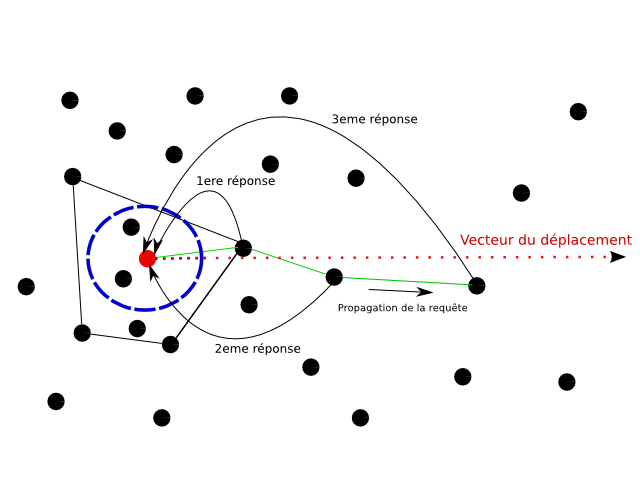
\includegraphics[scale=0.5]{../Images/propagation_algo.png}\\
        \caption{Algorithme de propagation}
        \label{Propa_Algo}
        \end{figure}
        \vspace{5mm}
	\subsection{Expérimentations et Résultats}
		Le travail a été testé sur le simulateur à évènement discret PeerSim ~\cite{peersim}, les expérimentations ont eu pour objectif de comparer Sollipsis avec et sans Blue Banana.
		\subsubsection{Le simulateur PeerSim}
		PeerSim est un simulateur de réseau pair à pair, qui a deux modes de fonctionnement: par cycles ou par évènements. C'est une API riche et modulaire qui est codée en Java, c'est un composante du projet BISON de l'université de Bologne (Italie). Ce simulateur permet de simuler un large nombre de machines et de tester différentes configurations du réseau. Le simulateur va faire des simplifications sur les couches réseau et les contraintes physiques (latence, pannes, ...). Chaque nœud est considéré comme un module qui va échanger des messages avec les autres nœuds du système. La plupart des plateformes de simulation sont basés sur le modèle à évènements discrets, il est possible de distinguer deux entités: les nœuds et les messages. Le temps va seulement évoluer à chaque nouvel évènement sur un nœud.
		\subsubsection{Description des expérimentations}
		Au départ de la simulation, une carte initiale des traces est introduite dans le simulateur. Ensuite, le simulateur va initialiser l'overlay de Sollipsis et vérifier que les deux règles de Sollipsis sont bien respectés sur chaque nœud, nous insérerons ensuite le reste des traces. Il faut aussi régler les différents paramètres du simulateur ( nombre d'avatar, surface du monde, densité, accélération des avatars, vitesse de connection ...). Plusieurs métriques sont mises en place pour évaluer les résultats:
	\begin{itemize}
	\renewcommand{\labelitemi}{$\bullet$}
		\item \textit{Violation of Solipsis fundamental rules}: Regarde si les propriétés de \textit{Global Connectivity} et de \textit{Local Awareness} sont respectées.
		\item \textit{Knowledge of nodes ahead of the movement}: Mesure pour les avatars qui se déplacent rapidement, le temps moyen pour qu'il connaisse un nœud qui sera sur sa trajectoire.
		\item \textit{Exchanged messages count}: Mesure l'impact de Blue Banana sur le réseau, cela va compter le nombre de message introduit par Blue Banana et Sollipsis.
	\end{itemize}
		\subsubsection{Les résultats}
		Les des résultats les plus intéressants sont que Blue Banana diminue les transition en échec de 55\% à 20\%, augmentent la connaissance des prochains nœuds de 270\% et cela en créant un overhead de seulement 2\%. Les résultats montrent que le mécanisme d'anticipation introduit par Blue Banana aide l'overlay de Sollipsis à s'adapter à temps et à réduire significativement le nombre de violation des règles de Sollipsis ( de 55\% ou 80\% à 20\%). 
